\chapter{LapOps Application}\label{manual}
This section describes, explains and shows the application that was created in this workshop. It contains a manual and additional informations for the correct usage of LapOps.

\section{LapOps Manual}
The following section describes how the user can interact with LapOps and what the user needs to do, to use it properly.

\subsection{Preparation}\label{prep}
Because we chose the near field sensor to keep track of our laps, it is necessary to create a bridge, or start/finish line, that is close enough to the device if the car travels through it. The distance between the bottom of the bridge and the device has to be less than 4 centimetres. To confirm if the distance is small enough you can refer to our application. The pictures visible in figure \ref{LabOpsnearfield} show LapOps, when it needs to be put at the starting line. The GO button only appears when the near field sensor is active and therefore the laps can be started. It also signals a successful preparation.

\begin{figure}[H]
	\centering
	\includegraphics[scale= 0.1]{Pictures/bridgedistance.png}
	\caption{RC car with mounted device and bridge for a start/finish line}
	\label{startFinishLineWithRC}
\end{figure}

\begin{figure}[H]
	\begin{subfigure}[c]{0.4\textwidth}
		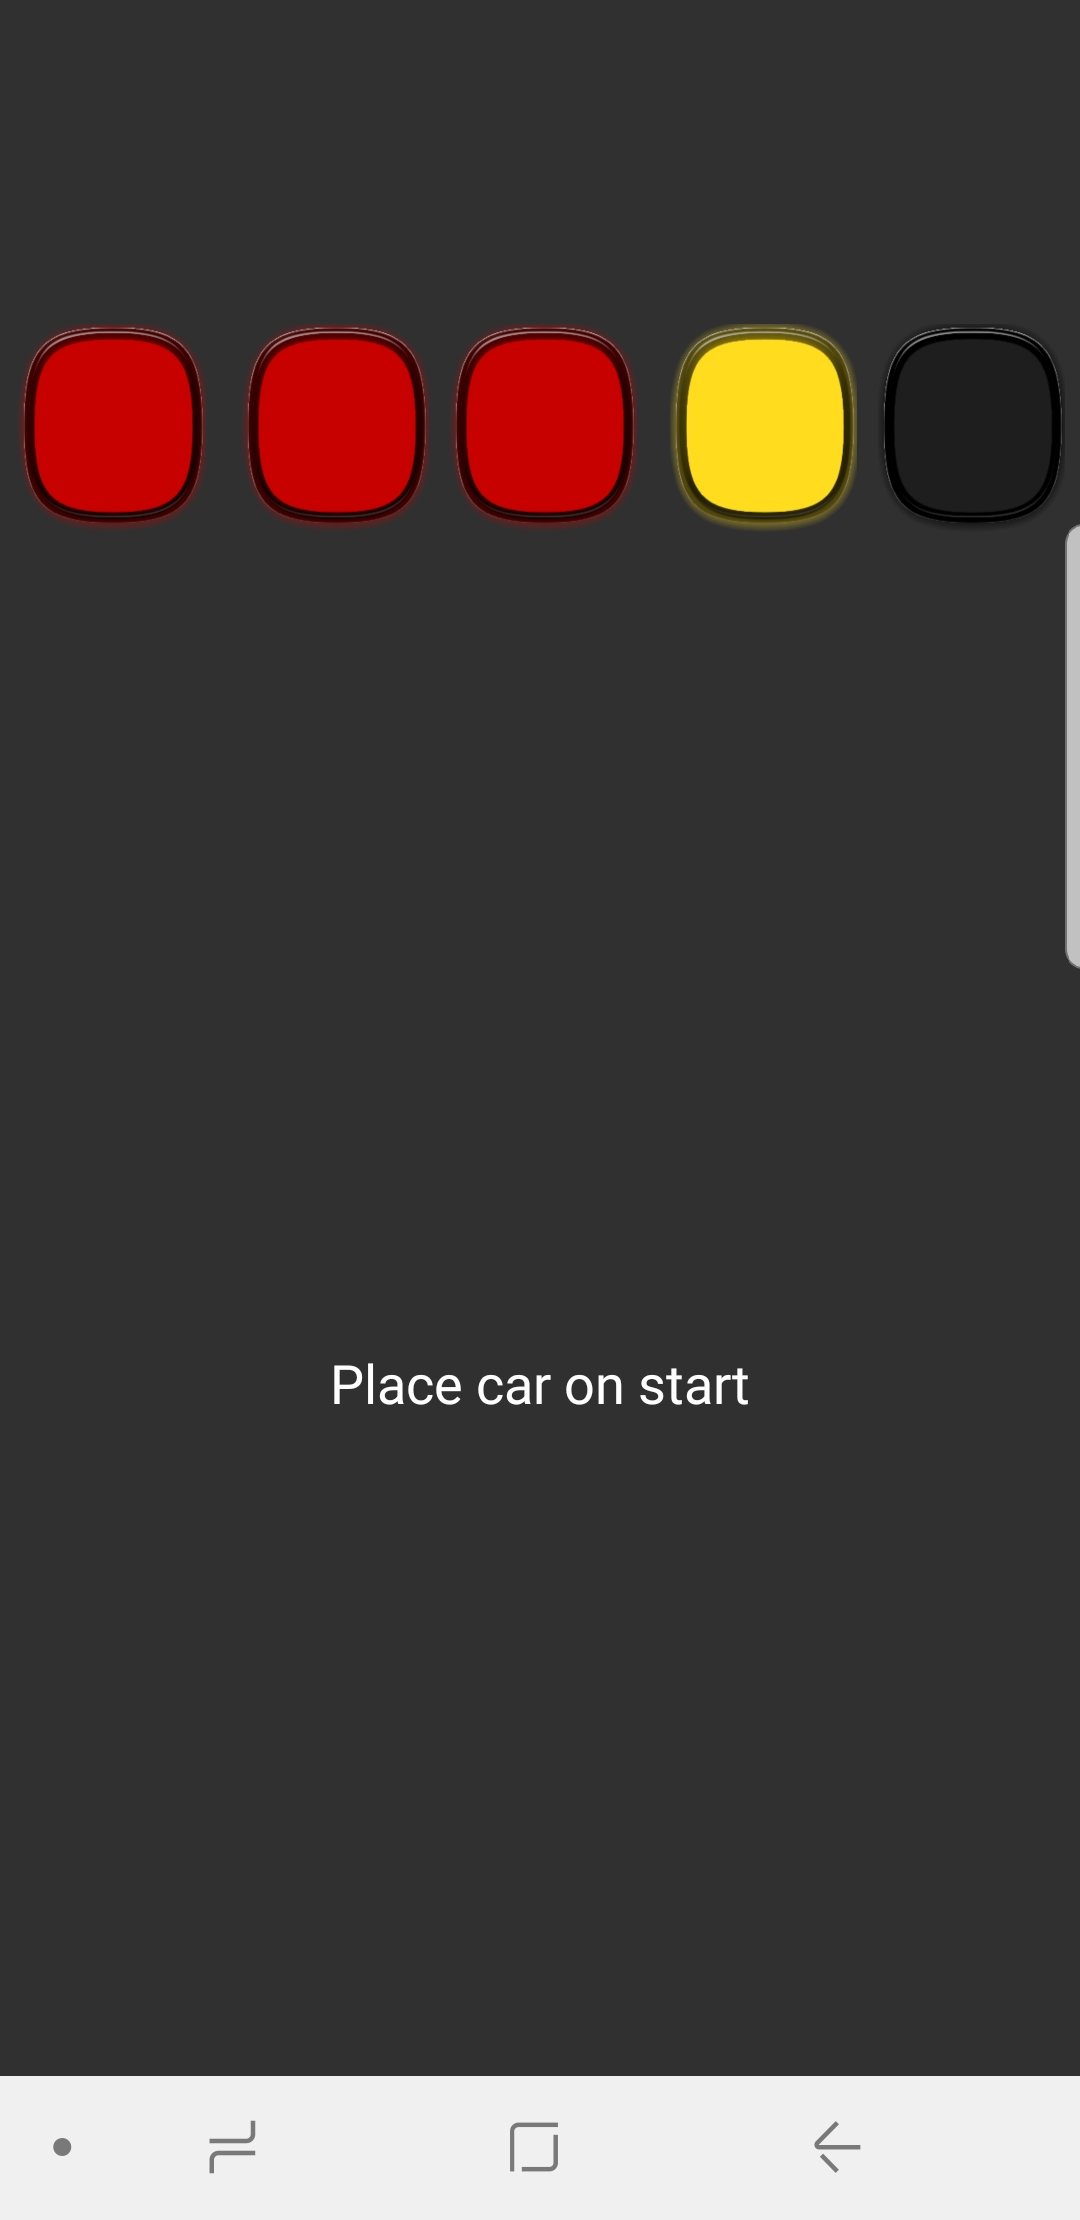
\includegraphics[width=\textwidth]{Pictures/App/PreNearFiled.jpg}
		\subcaption{Car needs to be put in position to activate near field sensor}
		
	\end{subfigure}
	\hfill
	\begin{subfigure}[c]{0.4\textwidth}
		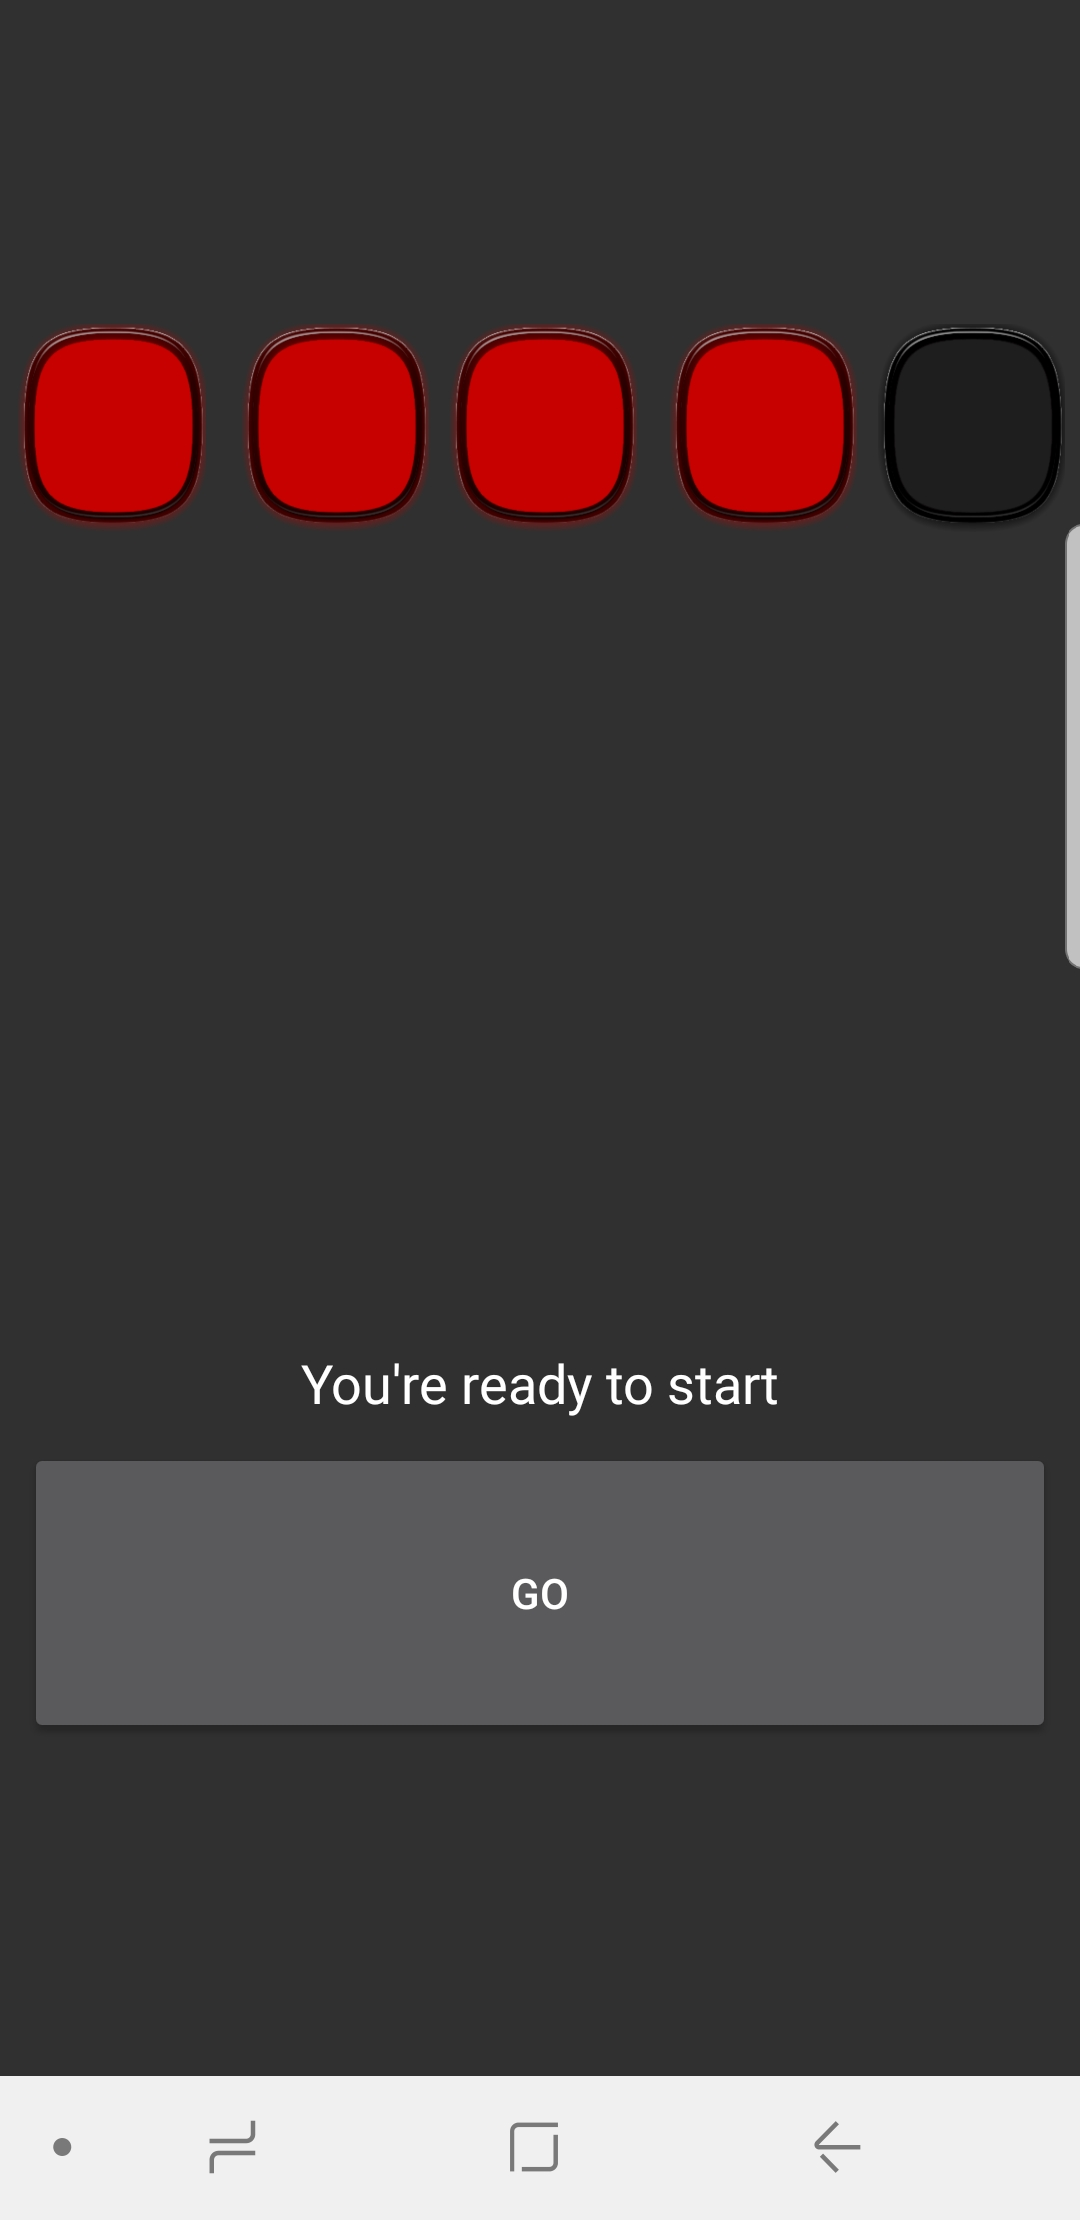
\includegraphics[width=\textwidth]{Pictures/App/FieldActivated.jpg}
		\subcaption{Near field sensor is activated and LapOps is ready to collect data}
		
	\end{subfigure}
	\caption{Overview of LapOps for starting phase}
	\label{LabOpsnearfield}
\end{figure}

\subsection{LapOps Usage}
After doing the preparation steps in section \ref{prep} it is pretty easy to use LapOps. The only thing that needs to be done is driving on a defined track that can be chosen freely. Please consider, that enough laps need to be driven for the system to recognize a pattern in the accelerometer data. In our tests 10 to 15 laps were mostly fine. After driving the laps, just stop the car and click on the finish button. After processing of the data, the result screen will be displayed. The first thing, that is visible will be the screen seen in figure \ref{LapOpsResult} (a). This overview lists all the driven laps and their state. Green represents the fastest lap in the current session. Yellow represents laps, that are valid. These can be opened to view the performance of the sections. The red laps are considered invalid. That happens if the track that the car drove was too different from the rest. After clicking on a valid lap (yellow) the screen visible in figure \ref{LapOpsResult} (b,c) will be visible. In this overview, the yellow represents a result in the same range to the fastest lap. The red color represents slower sections and the green one is there to indicate a faster section compared to the fastest lap.
\begin{figure}[H]
	\begin{subfigure}[c]{0.32\textwidth}
		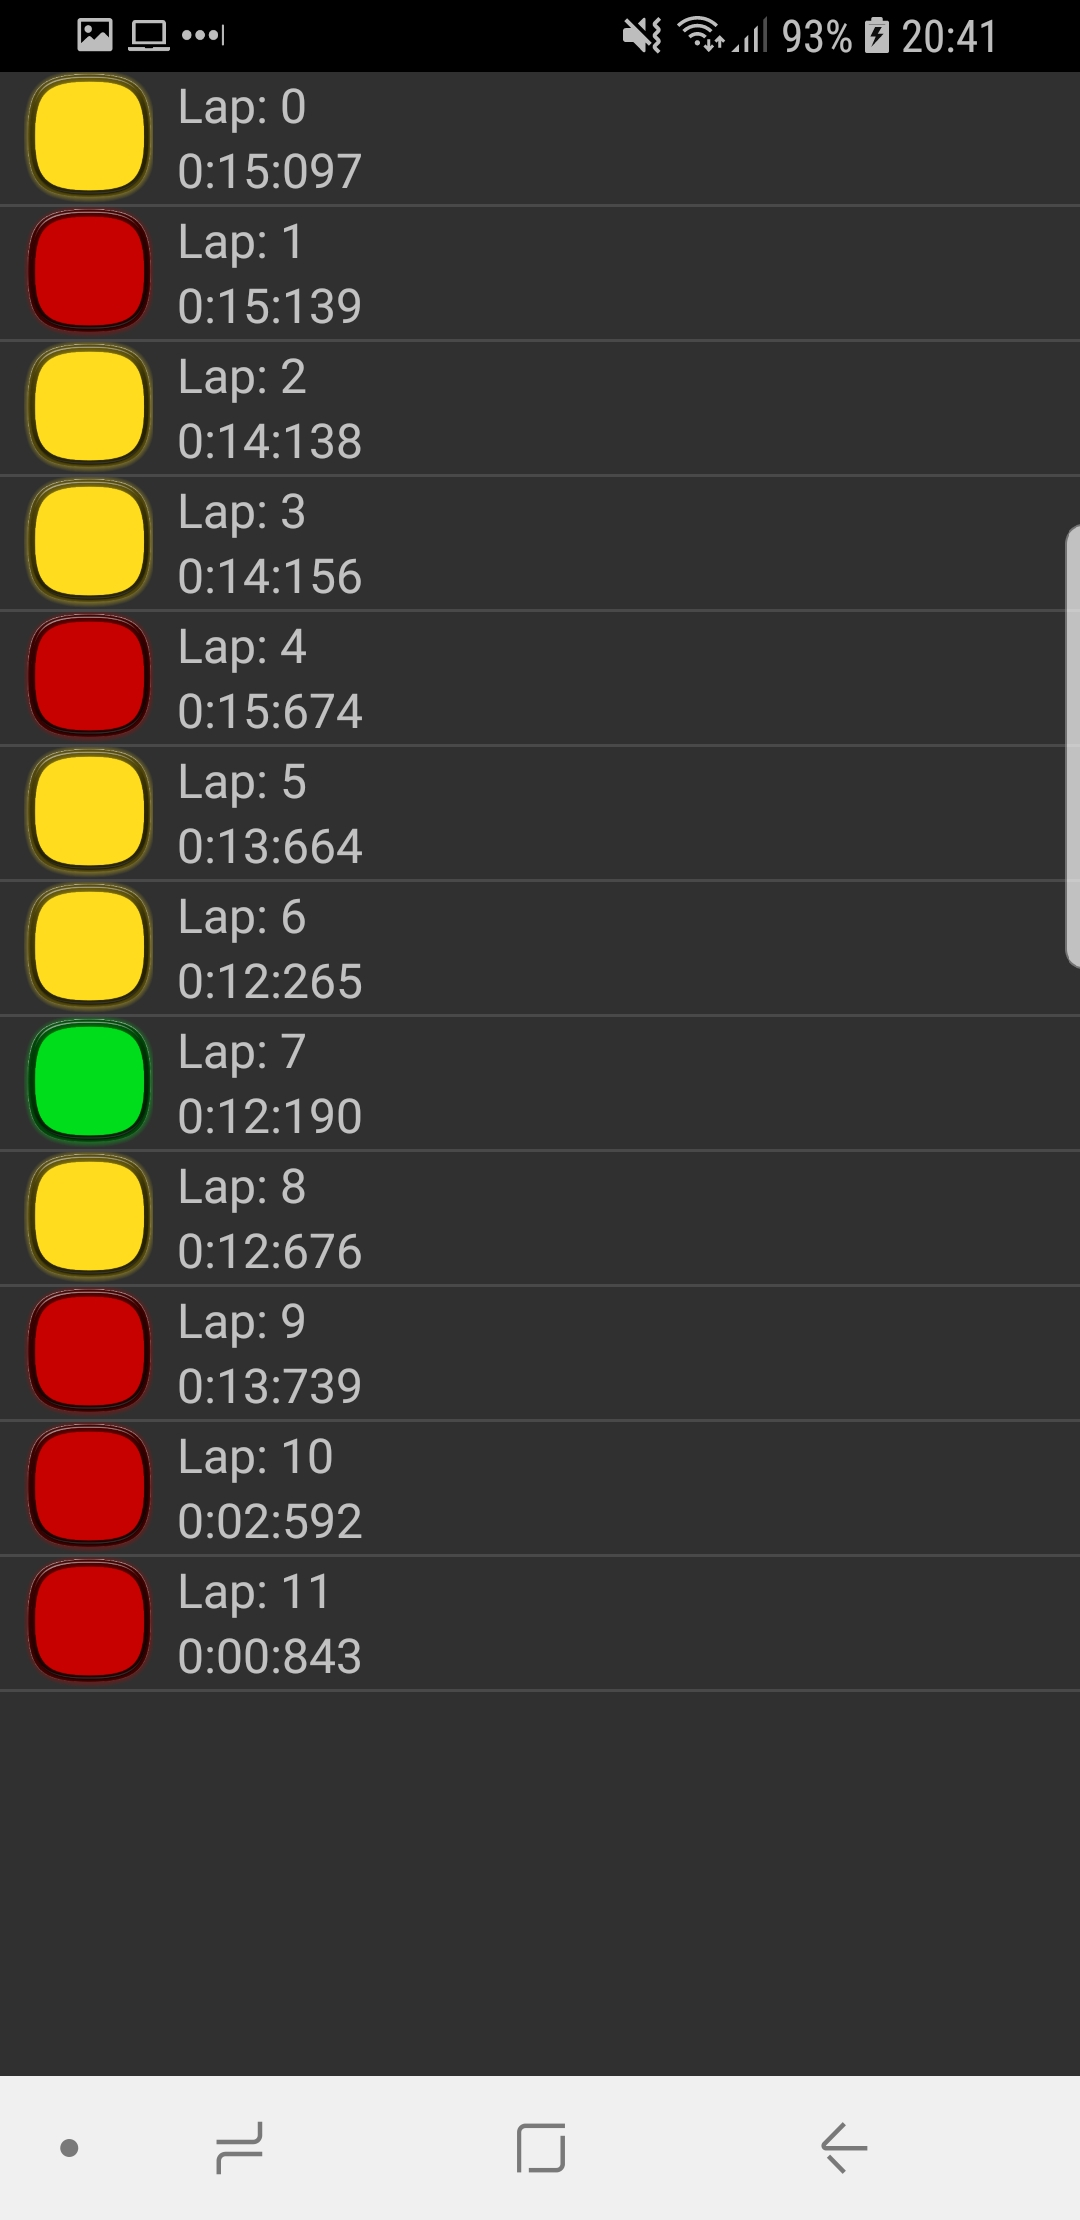
\includegraphics[width=\textwidth]{Pictures/App/LapList.jpg}
		\subcaption{Overview of the driven laps}
		
	\end{subfigure}
	\hfill
	\begin{subfigure}[c]{0.32\textwidth}
		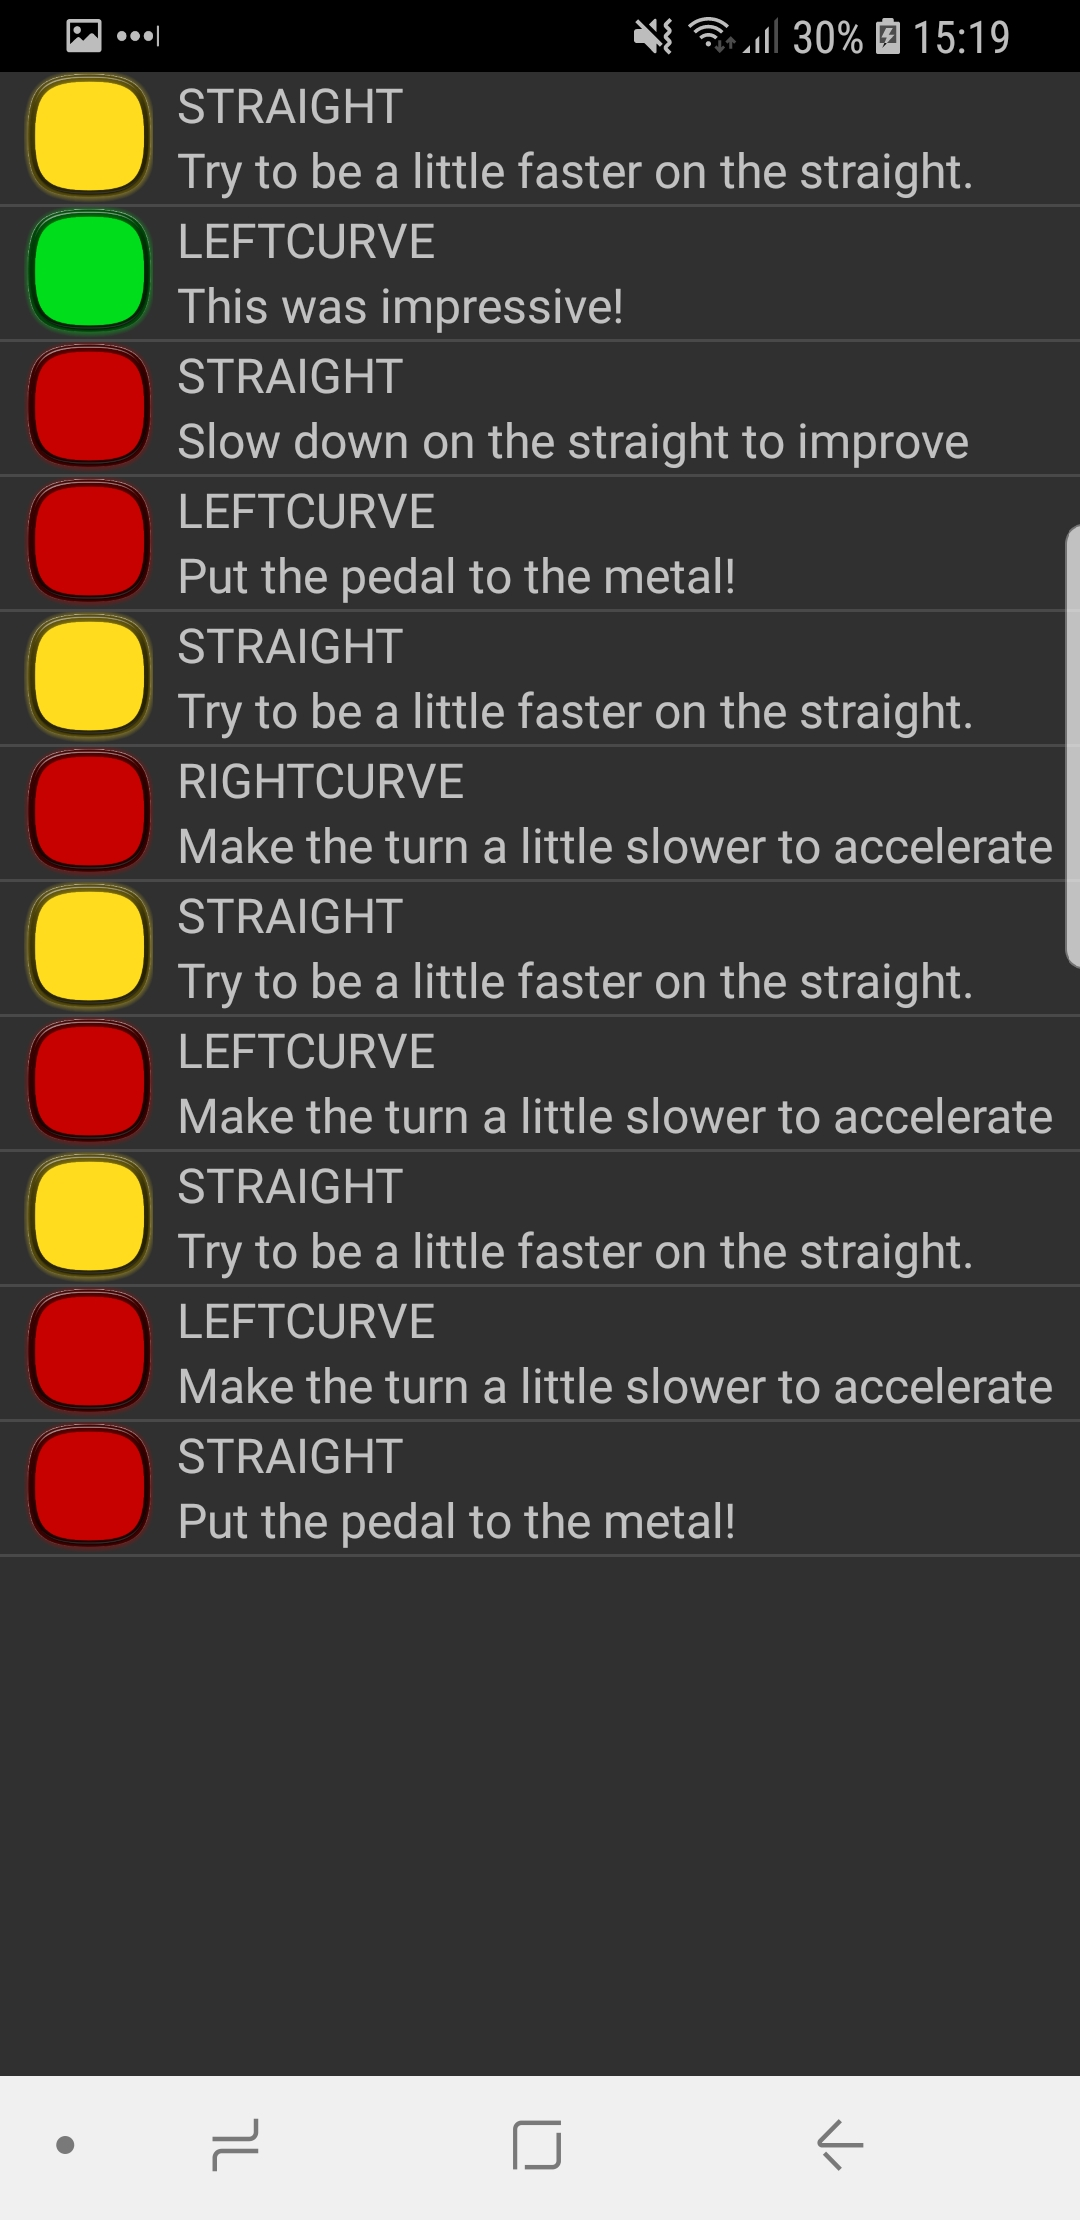
\includegraphics[width=\textwidth]{Pictures/App/SectionScreen1.jpg}
		\subcaption{Section overview of lap 3}
		
	\end{subfigure}
	\hfill
	\begin{subfigure}[c]{0.32\textwidth}
		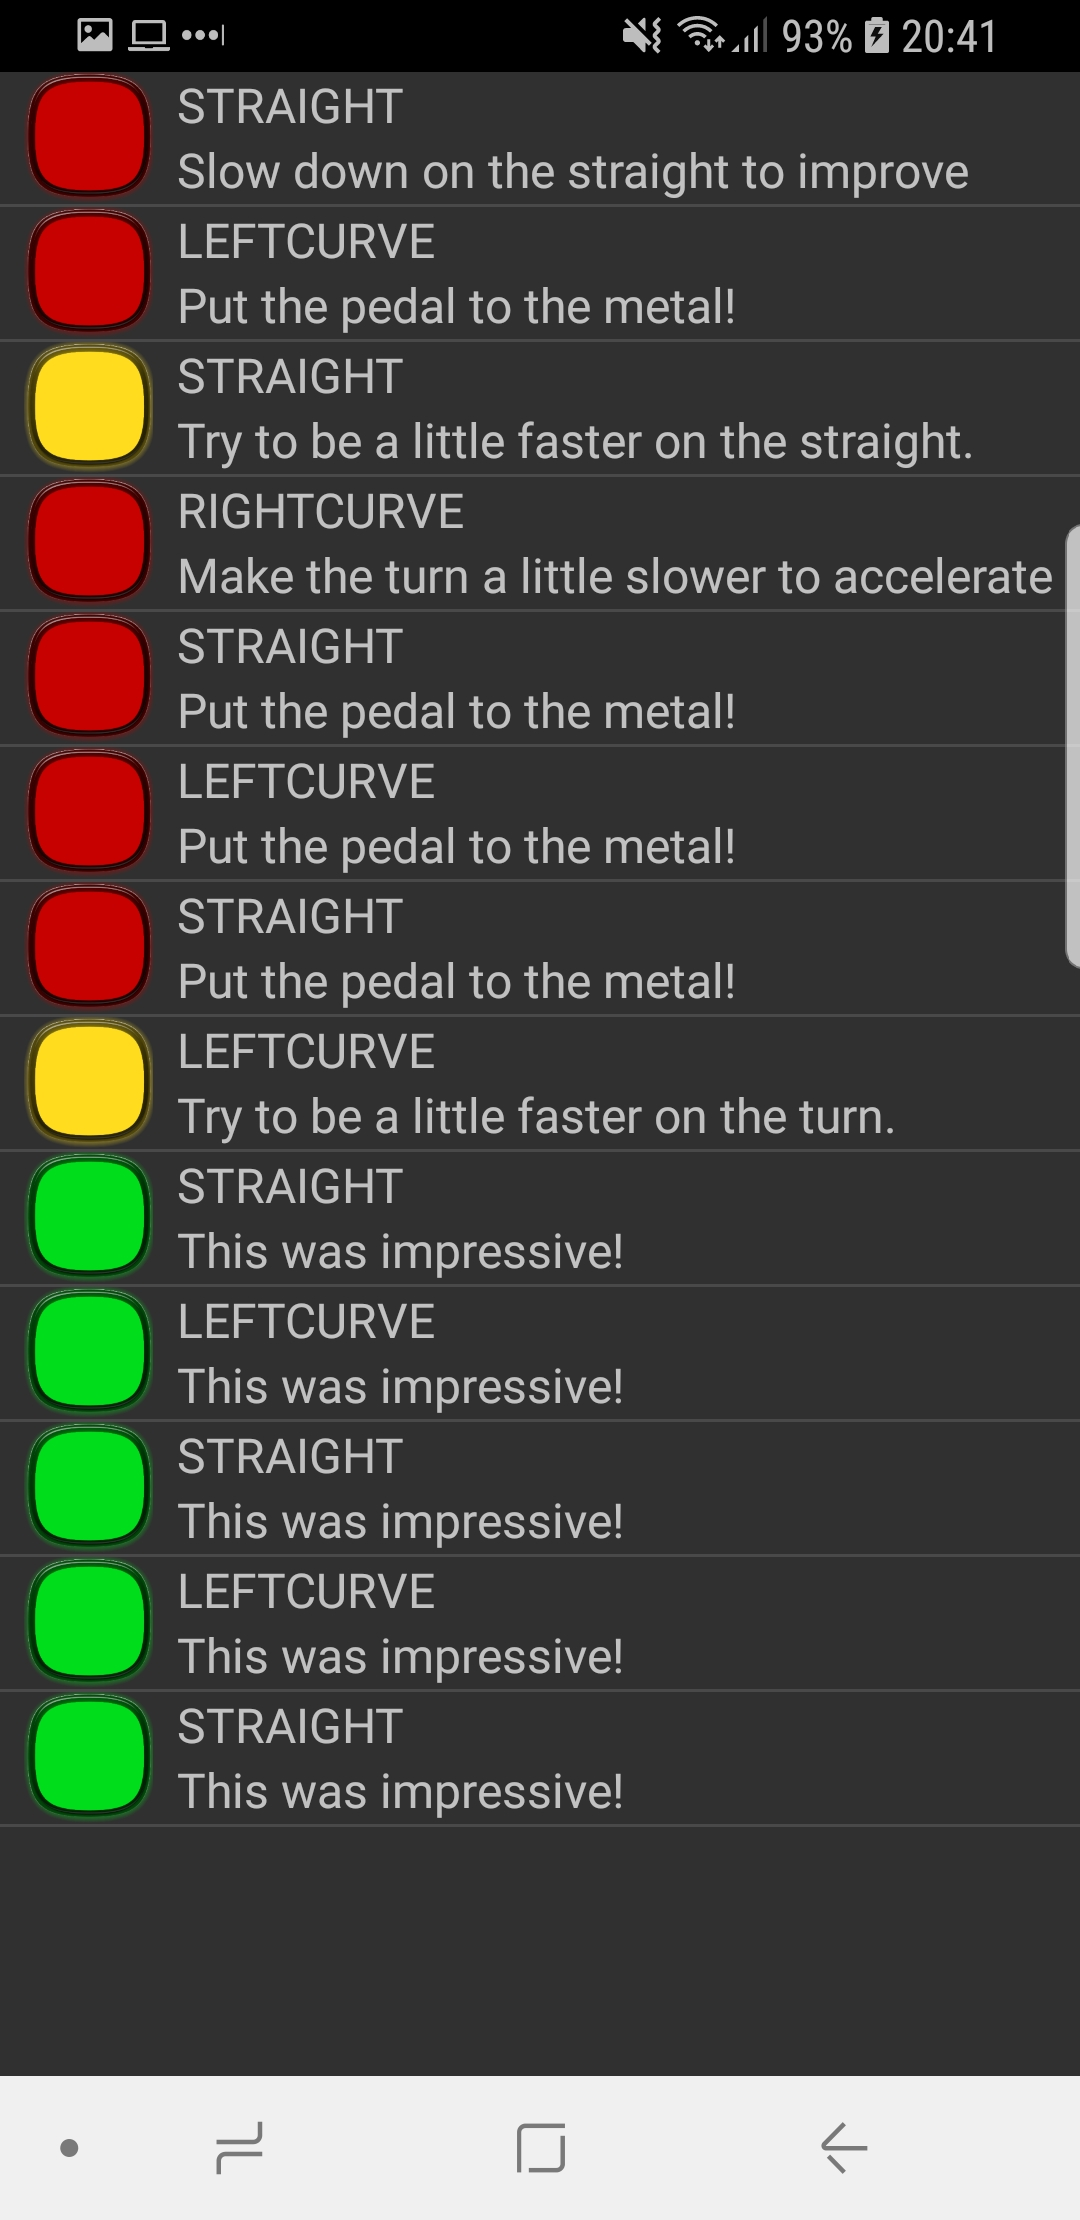
\includegraphics[width=\textwidth]{Pictures/App/SectionScreen2.jpg}
		\subcaption{Section overview of lap 9}
	\end{subfigure}

	\caption{Result screens of LapOps}
	\label{LapOpsResult}
\end{figure}
\newpage
\section{Additional Information}
This section provides additional information of the project. 

\subsection{Issues with Provided Smartphone}
One big issue was the near field sensor of the provided Huawei smarthphone. The near field sensor is heavily delayed and does not register if driven to fast under the bridge. Therefore if there is a need to use the Huawei smarthphone please drive very slowly under the bridge for the near field sensor to trigger. 

\subsection{Login for the Different Social Channels}
The following section lists the login credentials for the social channels, that were used in this project. For the passwords refer to the printed version.
\begin{figure}[H]
	\centering
	\begin{tabular}{ l | p{5.6cm} | p{5.6cm} }
		Website & Login & Link \\ \hline
		youtube.com & Login: dsce.team.d@gmail.com Pw: ******* & https://bit.ly/2Htqy7n\\
		hackster.io & Login: dsce.team.d@gmail.com Pw: ******* & https://bit.ly/2r0Em28 \\
	\end{tabular}
\end{figure}
\newpage
\subsection{Test Data and Corresponding Tracks}
The provided Huawei smartphone is preloaded with four test datasets, that are also located in the dataset folder. For visualization purposes all tracks are drawn in this section.
\begin{figure}[H]
	\centering
	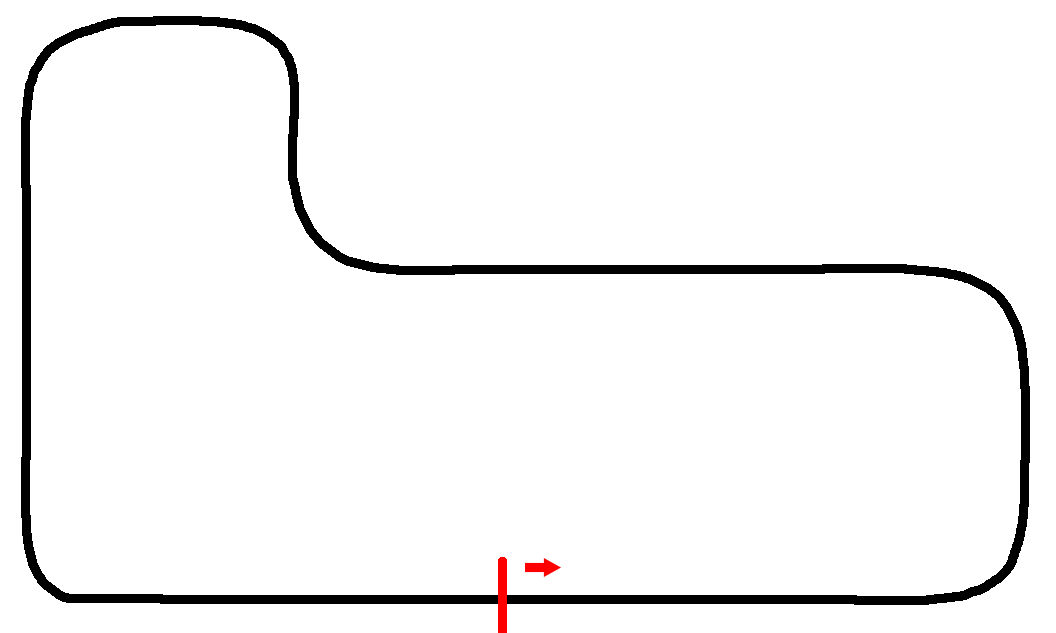
\includegraphics[scale= 0.5]{Pictures/Basic1.png}
	\caption{Layout for the dataset Basic1 and Basic3}
	\label{Basic1}
\end{figure}
\begin{figure}[H]
	\centering
	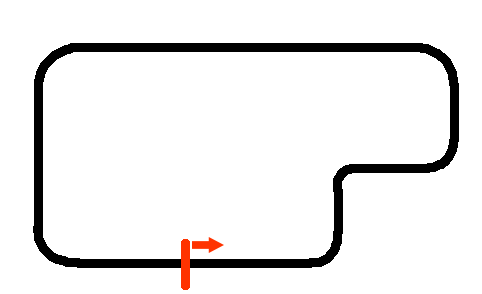
\includegraphics[scale= 1]{Pictures/Basic2.png}
	\caption{Layout for the dataset Basic2}
	\label{Basic2}
\end{figure}
\begin{figure}[H]
	\centering
	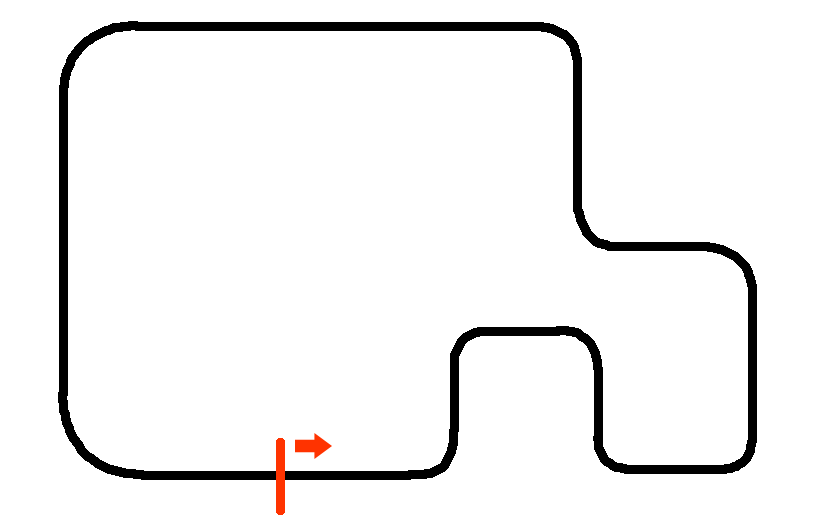
\includegraphics[scale= 0.5]{Pictures/Complex.png}
	\caption{Layout for the dataset Complex}
	\label{Complex}
\end{figure}


